There are two fundamental causes that can impede the I/O performance in an extreme-scale SSIO system. One is indirection, where layers of storage tiers are employed either for performance and/or for scalability reasons.  The direct consequence is that there could be multiple traversing paths from application end to the rest place of data, and more often than not, the I/O paths are not under control under any single authority. The other cause is the shared use of resources. The best effort I/O request/response nature and lack of QoS mechanisms imply that there is little guarantee in terms of expected performance.  Both indirection and shared use of resource contribute to a high probability of imbalanced use of resources thus the occurrence of congestion and degraded performance. Traditionally, there is a disconnection between storage infrastructure and rest of system software and applications: the infrastructure details are not exposed anywhere at all. One argument favoring this is to ensure a platform agnostic design. 

As an example to demonstrate that this disconnection will hurt system performance: We launch 4096 processes with each process doing a single file I/O operation against half of the Spider II file system. The traces of those files are analyzed to examine the utilization distribution of different components. Figure (a), (b) and (c) shows the resource usage distribution for OSTs, OSSes, and LNETs, respectively. We observe that there exists a significant variation in usage across components of any given type (e.g., OST, OSS or LNET). For example, some OSTs are used more than 10 times while some others are never used (corresponding to zero frequency count). Similarly, OSSes and LNETs show significant imbalance in usage under the default placement strategy. Consequently, imbalanced resource utilization increases the contention at certain components more than others. 

Given these insights, we advocate the idea that the infrastructure knowledge should find a way to relay to the upper layer for better and more effective use of resources.   We think this is more pertinent and critical given the recent development of multi-tier storage and storage component heterogeneity.  There needs to be a way for application/middleware layer to gain more exposure of storage system for more intelligent processing logic.  One prime example of such exposed knowledge can be request/response time. To most applications, this is a black box. Profiling it at the upper layer is neither efficient nor effective, as it doesn't reflect cross-layer characteristics. However, Most of storage layer does keep a detailed profiling of such information. We therefore envision and propose a histogram-based request/response profiling API that application and middleware layer can leverage and make more informative decisions.

\begin{figure}[tbh]
  \centering
  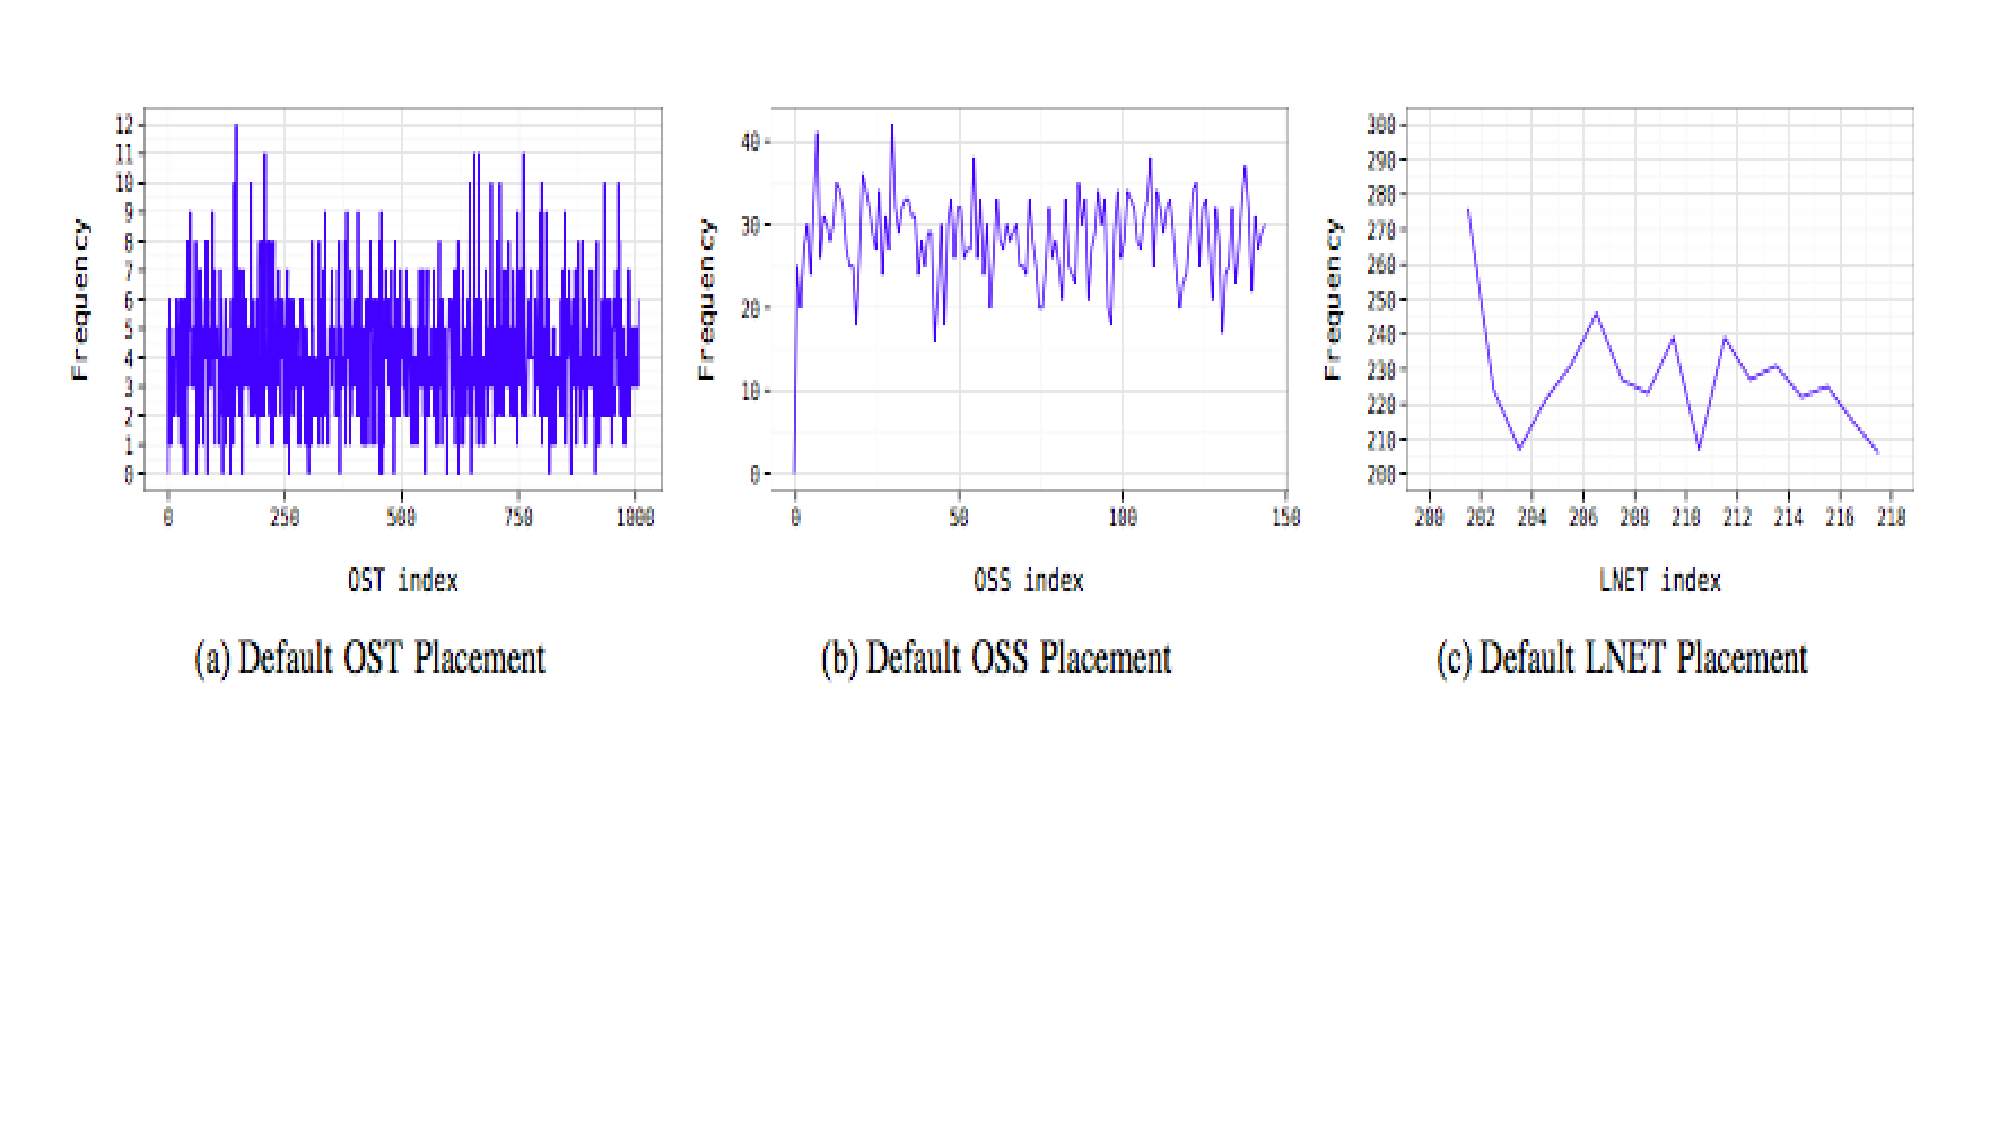
\includegraphics[width=\columnwidth]{graphics/infrastructure.pdf}\vspace{-1.2in}
  \caption{Resource usage distribution for OST(a), OSS(b) and LNETs(c). }
\end{figure}

%%% Local Variables:
%%% mode: latex
%%% TeX-master: "../proposal"
%%% End:
